The energy detector in (\ref{eq:energy_detector}) may be generalized by adding a
non-negative weight to each component in the sum. The statistic for the
weighted energy detector is 
\beq\label{eq:weighted_detector}
\Lambda_{\text{weighted}}(w) = w^TAw = \sum_{i=1}^k a_iw_i^2.
\eeq
where $A=\diag(a_1,\dots,a_k)\in\reals^{k\times k}$ and $a_i\geq0$. We constrain $\sum_{i=1}^k a_i = 1$ so that the weights
reside on the $(k-1)$-simplex. This reduces the set of possible weights by eliminating
those that are multiples of each other, which results in equivalent
detectors. The weighted energy detector gives practitioners additional design freedom to
maximize detector performance. Using a similar analysis as in Section
\ref{sec:energy_detector}, the conditional distributions of the weighted energy detector's 
statistic in (\ref{eq:weighted_detector}) are
\beq\label{eq:roc_weighted}
\ba
&\Lambda(w)|H_0\sim\sum_{i=1}^k a_i\chi_{1i}^2,\\
&\Lambda(w)|H_1\sim\sum_{i=1}^k a_i \chi_{1i}^2\left(\delta_i^2\right),
\ea
\eeq
where $\chi_{1i}^2$ are independent chi-square random variables with one degree of freedom
and $\chi_{1i}^2\left(\delta_i^2\right)$ are independent non-central chi-square random variable
with one degree of freedom and non-centrality parameter $\delta_i^2$. We can relate $P_D$
to $P_F$ using the expression
\beq\label{eq:weighted_pd}
P_{D_{\text{weighted}}}(P_F,A) = 1 - Q_{\Lambda|H_1}\left(Q^{-1}_{\Lambda|H_0}(1-P_F)\right)
\eeq
where $Q_{\Lambda|H_1}$ is the c.d.f of $\Lambda(w)|H_1$ in (\ref{eq:roc_weighted})
and $Q_{\Lambda|H_0}$ is the c.d.f. of $\Lambda(w)|H_0$ in (\ref{eq:roc_weighted}). 

The definition of $\Lambda_{\text{weighted}}(w)$ in (\ref{eq:weighted_detector}) raises
the natural question 
\begin{quote}
  Given $\delta$ and a desired $P_F$, what is the optimal choice of weighting matrix, $A$,
  that maximizes $P_{D_{\text{weighted}}}(P_F)$ for a weighted energy detector with the
  form of (\ref{eq:weighted_detector}) using observations generated from
  (\ref{eq:general_setup})?
\end{quote}
While the c.d.f. of chi-square and non-central chi-square random variables are known in
closed form, the c.d.f. of a weighted sum of chi-square random variables is not known in closed
form and therefore (\ref{eq:weighted_pd}) cannot be computed analytically. It is common
to use saddlepoint approximation techniques \cite{wood1993saddlepoint} to compute the
c.d.f. of such sums in (\ref{eq:roc_weighted}), however, such techniques must be computed
for many thresholds, $\eta$, to generate a ROC curve for one weighting matrix $A$. To
optimize over $A$ in (\ref{eq:weighted_pd}), this process would need to be repeated over a
discretization of the ($k-1$)-simplex. Developing a more efficient algorithm to optimize
over the weighting matrix, $A$, is an important topic for future work.

To illustrate how weighted energy detectors can improve detection performance, consider a rank-2 setting where the desired
false alarm rate is $P_F=0.1$. Optimizing $A=\diag(a_1,a_2)$ on the simplex $a_1+a_2=1$
results in one degree of freedom and so
\be
\Lambda(w)_{\text{weighted}} = aw_1^2 + (1-a)w_2^2  
\ee
where $a\in[0,1]$. Figure \ref{fig:weighted} plots the empirically achieved (see
\cite{fawcett2006introduction}) probability of detection as a 
function of the weighting parameter $a$ for four detectors each with a different signal
vector $\delta$. Figure \ref{fig:weights_easy} shows results for detectors using
$\delta=[1,1]^T$ and $\delta=[1,0]^T$. The detector with $\delta=[1, 1]^T$ achieves
maximum performance when $a=0.5$, which weights both components equally. As
$\delta_1=\delta_2=1$ both $w_1$ and $w_2$ have the same conditional distributions and it
is intuitive that we weight both components equally. However, the detector using
$\delta=[1, 0]^T$ achieves maximum performance when $a=1$ indicating that the second
component is not useful in detection. As $\delta_2=0$, $w_2$ has the same distribution
under both the $H_1$ and $H_0$ hypotheses, giving it no discriminatory power. For these
values of $\delta$, the optimal $a$ is obvious and the performance of the weighted energy
detector is the same as that of the standard energy detector.

\begin{figure}[t]
\centering
\subfigure[Easy Optimal Weights]{
  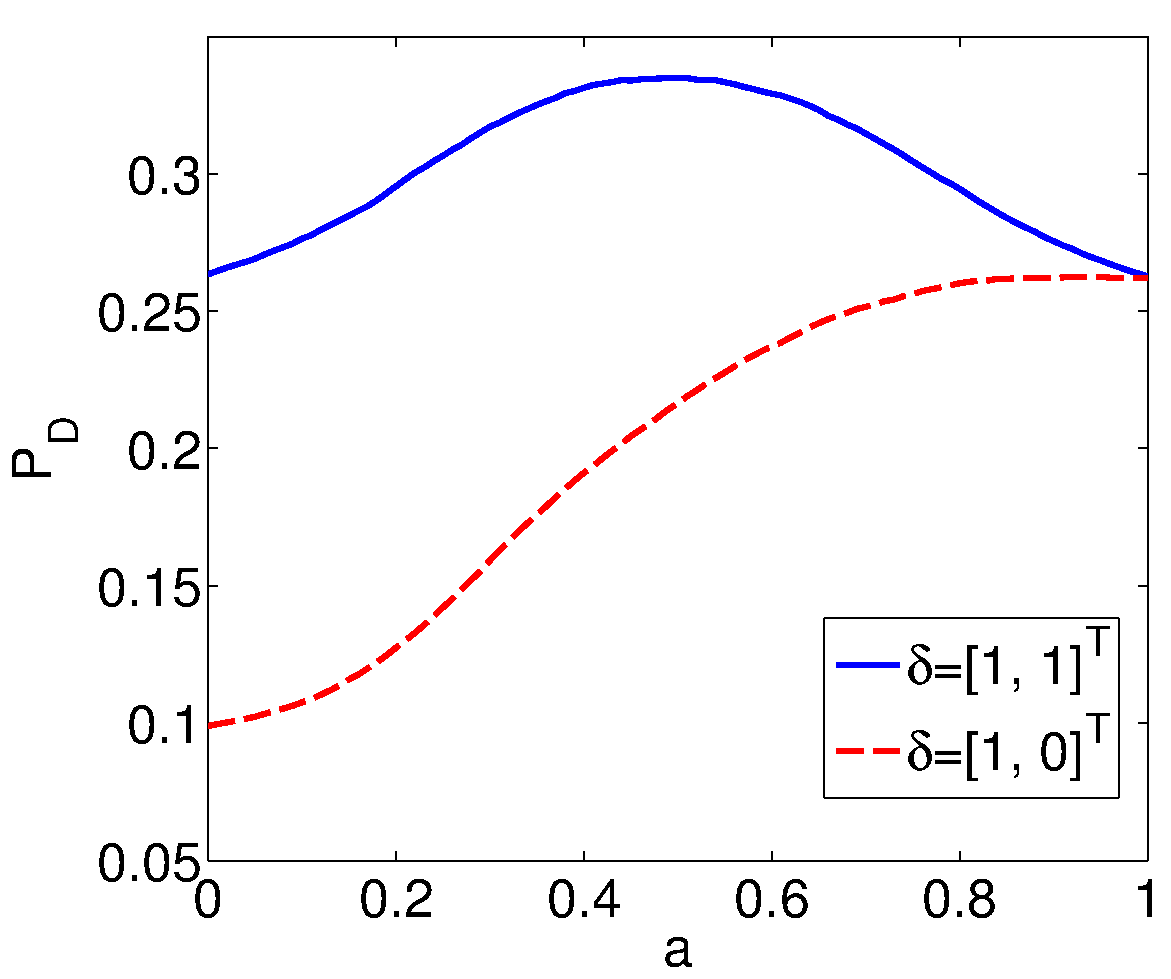
\includegraphics[width=0.45\textwidth]{taes_msd/figures/weights_easy.pdf}
  \label{fig:weights_easy}}
\subfigure[Difficult Optimal Weights]{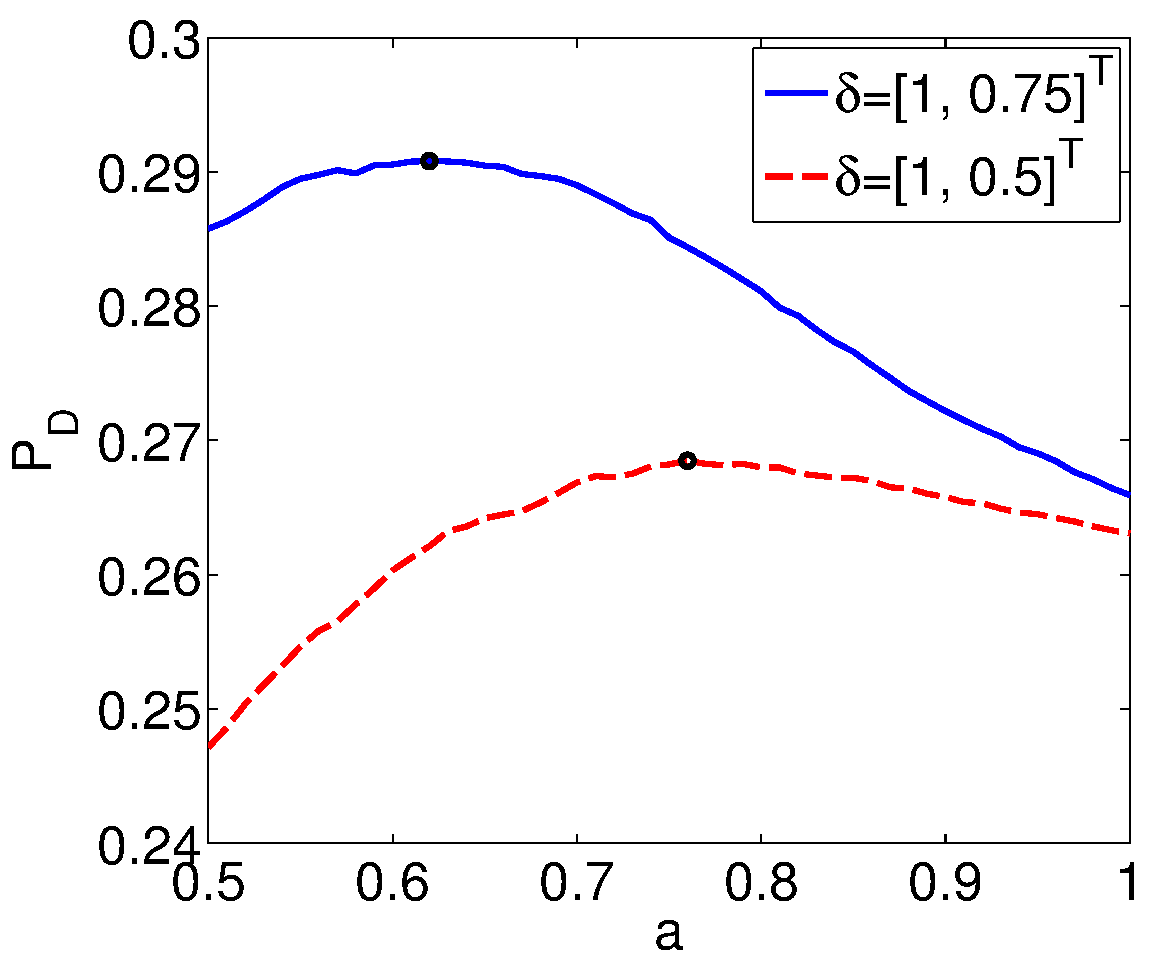
\includegraphics[width=0.45\textwidth]{taes_msd/figures/weights_hard.pdf}
  \label{fig:weights_hard}}
\caption{Empirically achieved probability of detection ($P_D$) as a function of the
  weighting coefficient $a$ for a fixed false alarm rate of $P_F=0.1$. (a) Two detectors,
  one using the deterministic vector $\delta=[1,1]^T$ and the second using
  $\delta=[1,0]^T$.  The first detector achieves its maximum performance around $a=0.5$
  indicating that both components are equally informative. The second detector achieves
  its maximum performance at $a=1$ indicating the second subspace component is not useful
  in detection. (b) Two detectors, one using $\delta=[1, 0.75]^T$ and the other using
  $\delta=[1, 0.5]^T$. The maximum performance of each detector is no longer achieved at
  $a=0.5$ or $a=1$ as the entries of $\delta$ are non-zero and are not equal. The maximum
  performance is indicated by a black circle.}
\label{fig:weighted}
\end{figure}


Figure \ref{fig:weights_hard} considers detectors using $\delta=[1, 0.75]^T$ and $\delta=[1,
0.5]^T$. Both choices place $\delta_1>\delta_2$ so we only consider the regime $a\in[0.5,
1]$, which weights the first component stronger than the second. The maximum performance
of each detector is indicated by a black circle. Unlike the detectors in Figure
\ref{fig:weights_easy}, the maximum $P_D$ is not achieved at $a=0.5$ or $a=1$; both
components are needed to achieve optimal performance. For these choices of $\delta$, the
weighted energy detector is able to achieve a better performance than a standard energy
detector using either one ($a=1$) or both ($a=0.5$) components. Developing an efficient algorithm
to compute these optimal weights is an important extension of the work in this chapter.
